\documentclass[a4paper,12pt]{article}
\usepackage[utf8]{inputenc}
\usepackage[english]{babel}
\usepackage{graphicx}
\DeclareGraphicsExtensions{.pdf,.png,.jpg}
\usepackage{listings}
\usepackage{hyperref}
\lstset{
language=C,
basicstyle=\footnotesize
}
\begin{document}

\section{Lab 1}
\subsection{Before the lab session}

\begin{itemize}
\item \textit{Write a detailed explatation why computation load can be imbalanced and how it affects the global performance.}

  Since different pixels can take different amounts of time to calculate, for example completely black pixels taking the maximum amount of allowed iterations, the pixels assigned to one thread might be quicker to process than those assigned to a different thread.

  The result of this being that the different threads being assigned the same number of pixels will have different execution times depending on if they get an area with majority black population or not.

  Since black pixels tend to flock together rather than appearing stocastically it's reasonable that one thread will get a heavier load than another.


\item \textit{Describe a load-balancing method that would help reducing the performance loss due to load-imbalance.}

Instead of giving each thread big areas, as described in Figure 4 of the lab compendium, one could assign each interleaving rows or columns of the image 1 pixel wide which should distribute the load more eavenly.

\end{itemize}



\subsection{During the lab}

We solved the issue by letting each thread compute one row at a time hoping that it would make for an even distribution of work. Doing it row-wise also means that the threads are accessing the array of pixels linearly which is condusive to caching.

Included below is a couple of graps demonstrating our intelligent load balancing.

\begin{figure}[h]
  \centering
  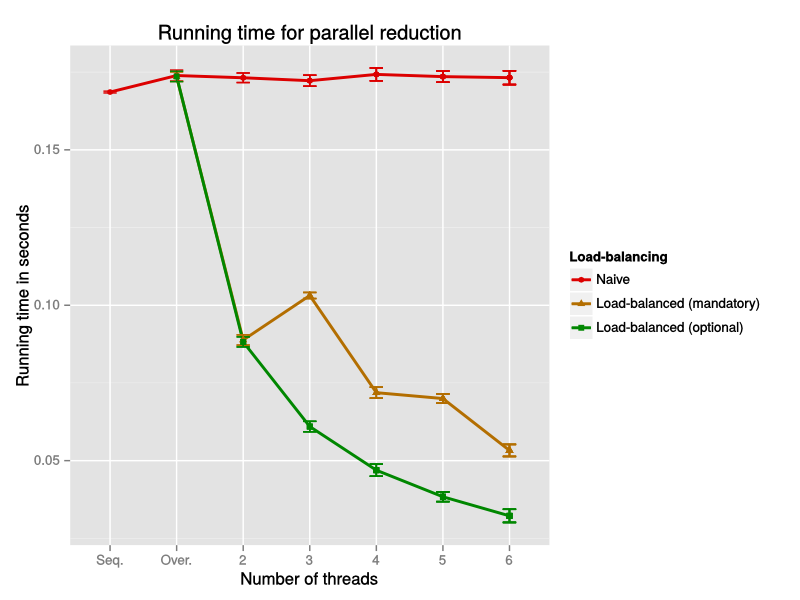
\includegraphics[width=0.9\textwidth]{1_timing.png}
  \caption{Comparison of no, naïve and intelligent load balancing.}
\end{figure}

\begin{figure}[h]
  \centering
  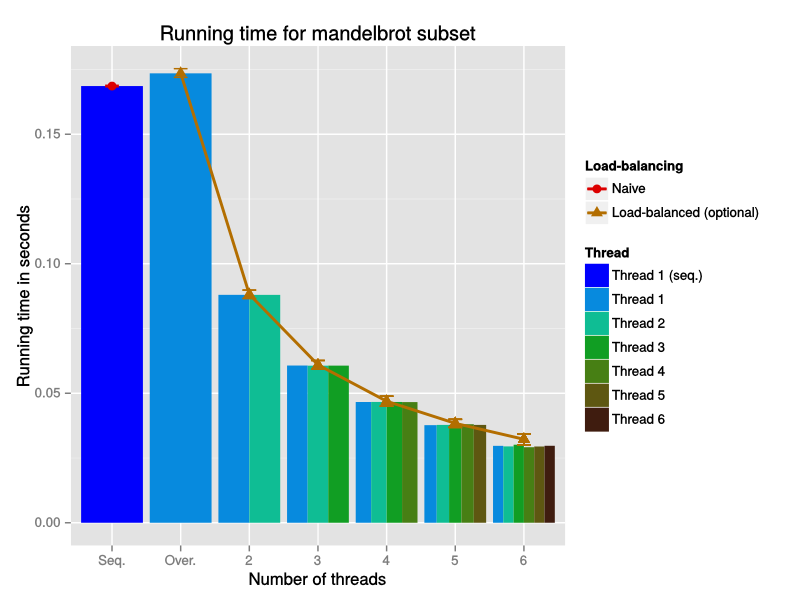
\includegraphics[width=0.9\textwidth]{4_timing-load_balance_2.png}
  \caption{Computational load per thread with the intelligent shader.}
\end{figure}

\end{document}